

%%% Local Variables:
%%% mode: latex
%%% TeX-master: "../../doktorarbeit"
%%% End:
\chapter{The effects of rotation}
In the previous chapter we studied four non-rotating models of core-collapse
supernovae, focusing on the underlying hydrodynamic instabilities responsible
for GW emission and how these excitation mechanisms change when taking the step from
2D to 3D. With this knowledge in hand, we will now discuss the effects of rotation.
In this chapter we present the GW signals from three core-collapse simulations of a 15 \msun  
progenitor \citep{heger_05}. Of the three simulations, two of the models include rotation
and in the third model rotation has been set to zero. This allows us allows us to study
how the GW signal changes, for the same stellar progenitor, with rotation.
Two of the three models (the fastest rotating model and the model without rotation)
are dominated by strong SASI activity, while the slowest rotating model only develops weak and intermittent SASI oscillations. 
This allows us to study the influence of rotation in both the SASI dominated regime and the convective regime. The model with the strongest
rotation successfully explodes and we can, therefore, also study the impact of rotation in the time after shock revival.

The study of GWs generated by the core-collapse of rotating stars
has a long and rich history. The first efforts consisted of idealised calculations, 
such as the rotating ellipsoidal models of \cite{thuan_74,novikov_76,shapiro_77,saenz_78,saenz_79,saenz_81}.
During the last four decades, starting in the early 80s with \cite{mueller_82}, the theoretical GW signals from multi-dimensional
simulations, with ever increasing sophisticatedness, have been extensively studied 
\citep{mueller_82,finn_90,moenchmeyer_91,yamada_95,zwerger_97,rampp_98,dimmelmeier_01,dimmelmeier_phd,
dimmelmeier_02_b,kotake_03,ott_04,yamada_04,shibata_04,cerda_05,saijo_05,ott_05,shibata_05,kotake_06,
obergaulinger_06b,ott_phd,dimmelmeier_07_a,dimmelmeier_07_bb,dimmelmeier_08,reisswig_11,
takiwaki_11,ott_12,kuroda_14,fuller_15}.

Rapidly rotating models are expected to have a strong GW burst associated with core bounce, 
see \cite{mueller_82} or  \cite{kuroda_14}, and \cite{fuller_15} for more recent results from 3D simulations.
During the time between core bounce and shock revival, very rapid rotation can cause
the inner core to deform in a bar-like manner \citep{rampp_98,shibata_05}.
In slower, but still fast, rotating models, 
a low-mode spiral instability has been found to develop 
\citep{ott_05,kuroda_14,takiwaki_16}. These instabilities leads to strong
GW emission that results in optimistic predictions of detection prospects.
The three models studied here are to slowly rotating to develop such instabilities 
and we will show that slow and moderate rotating progenitor does not yield the same
result and that detection with current GW detectors will be difficult, even for an
galactic event.

While slowly rotating models have not been well studied in 3D, there are several
indications that the rotation rate of core-collapse progenitors should be slow/moderate 
rather than rapid \citep{heger_05,beck_12,mosser_12,popov_12,noutsos_13,cantiello_14,deheuvels_14}. 
But, even slow rotation can help facilitate the success of core-collapse
simulations. The critical neutrino luminosity required to relaunch the stalled shock decreases when 
specific angular momentum is injected into the post-shock layer \cite{iwakami_14,nakamura_14}.
We find that, for the rotation rates studied here, there is no significant change to
the GW signal, compared to non-rotating models. While there are significant changes to the dynamics
and the underlying excitation processes of the GWs, the signal from our rotating models are not qualitatively
distinguishable from the non-rotating models studied in this thesis. 

This chapter is structured as follows: First, we present the numerical models and describe their dynamics,
we then give a description of the GW signals. In section~\ref{sec:p2ext} we describe the underlying hydrodynamic
effects responsible for GW excitation and discuss how they, and consequently the GW signals, are affected by rotation. 
Before we discuss our results and present our conclusion, we will assess the detection prospects of the three
models and what the effects of progenitor rotation are in this regard.  


\section{Supernova Models}
We present the GW signal from three models based on the progenitor of
\cite{heger_05}, which is a solar-metallicity star with a ZAMS mass of $15 \msun$.
The stellar evolution calculation took accounted for the effects of magnetic fields and rotation and
evolved the model from ZAMS to the onset of iron-core-collapse. The inclusion of magnetic fields leads to an overall
reduction of the final rotation rate of the iron core, compared to calculations without magnetic
fields \citep{heger_05}. 
The main difference between the three models is their rotation profiles. One of the models
uses the profile of the progenitor (m15r), one has an enhanced rotation profile (m15fr), 
and in the last model the rotation rate has been set to zero throughout the star (m15nr)
In \fig{figp2:rot} we show the rotation profiles of m15fr and m15fr.
\begin{itemize}
\item \textbf{m15fr:} The initial rotation profile of model m15fr was, by hand, set to a constant rotation rate of 0.5 rad/s
throughout the inner core of the star. At a radius of 1731 km the rotation profile was changed
to a linearly decaying profile (\fig{figp2:rot}). The model was simulated using the 
Yin-Yang grid, the two grid patches had an initial resolution of 400 cells, 56 cells and 144 cells in the radial, polar and
azimuthal directions, respectively. This corresponds to a 2 degree angular resolution. 
After the initial shock expansion halts around $60$ ms post bounce the average shock radius decreases slightly.
Between $\sim 80 - 160$ ms post bounce the shock front is more or less stationary. 
The shock starts to expand roughly $160$ ms after core bounce and soon after shock revival sets in.
In the time before shock revival, the post-shock flow is dominated by a strong spiral SASI mode. The SASI sets in around
$\sim 100$ ms post bounce.
\item \textbf{m15r:} The initial rotation profile of model m15r was exactly that of the progenitor \citep{heger_05}, without
any artificial changes made by hand. The rotation profile as a function of radius can be seen in \fig{figp2:rot}.  
The model was simulated using the Yin-Yang grid, the two grid patches had an initial resolution of 400 cells, 
56 cells and 144 cells in the radial, polar and azimuthal directions, respectively. This corresponds to a 2 degree angular resolution.
For the first $\sim 80$ ms after bounce, the evolution of the average shock radius of model m15r closely resembles that
of model m15fr. However, around $100$ ms after bounce the average shock radius starts to decrease. Unlike model m15fr, strong 
SASI activity does not develop in this model. The flow in the post-shock region is instead dominated by hot-bubble convection.
There is, however, some low amplitude dipole deformation of the shock front (see \fig{figp2:sasi}).
The average shock radius continue to decrease until
$\sim 200$ ms post bounce when the Si-O shell interface falls through the shock. The decreased density in front of the shock leads
to decreased ram pressure and a transient period of shock expansion. At $\sim 240$ ms post bounce the expansion subsides and
the shock front once more begins to retreat, a trend which continues until the end of the simulation.  
\item \textbf{m15nr:} In model m15nr the initial rotation rate was set to zero at all radii. The model was simulated using the Yin-Yang grid, the
two grid patches had an initial resolution of 400 cells, 28 cells and 72 cells in the radial, polar and
azimuthal directions, respectively. Which means that model m15nr was simulated with an angular resolution that is
two times coarser than the other two models (4 degrees). Initially, the shock expands and reaches a local maximum around $60$ ms after bounce,
from this point the shock radius steadily decreases until the Si-O shell interface falls through the shock. The decreased accretion rate
leads to a transient period of shock expansion until the shock eventually starts to recede once more. Except for the fact that
the average shock radius is generally larger in model m15nr, model m15nr is similar to model m15r in terms of the evolution of the average shock
radius. However, unlike model m15r, model m15nr develops strong SASI activity. In this model, the SASI activity is dominated by the sloshing mode.
The mode develops around $\sim 120$ ms after core bounce and peaks around $\sim 230$ ms post bounce. After the peak in activity 
the SASI mode gradually decays towards the end of the simulation.   
\end{itemize}
\begin{figure}[ht]           
\centering                            
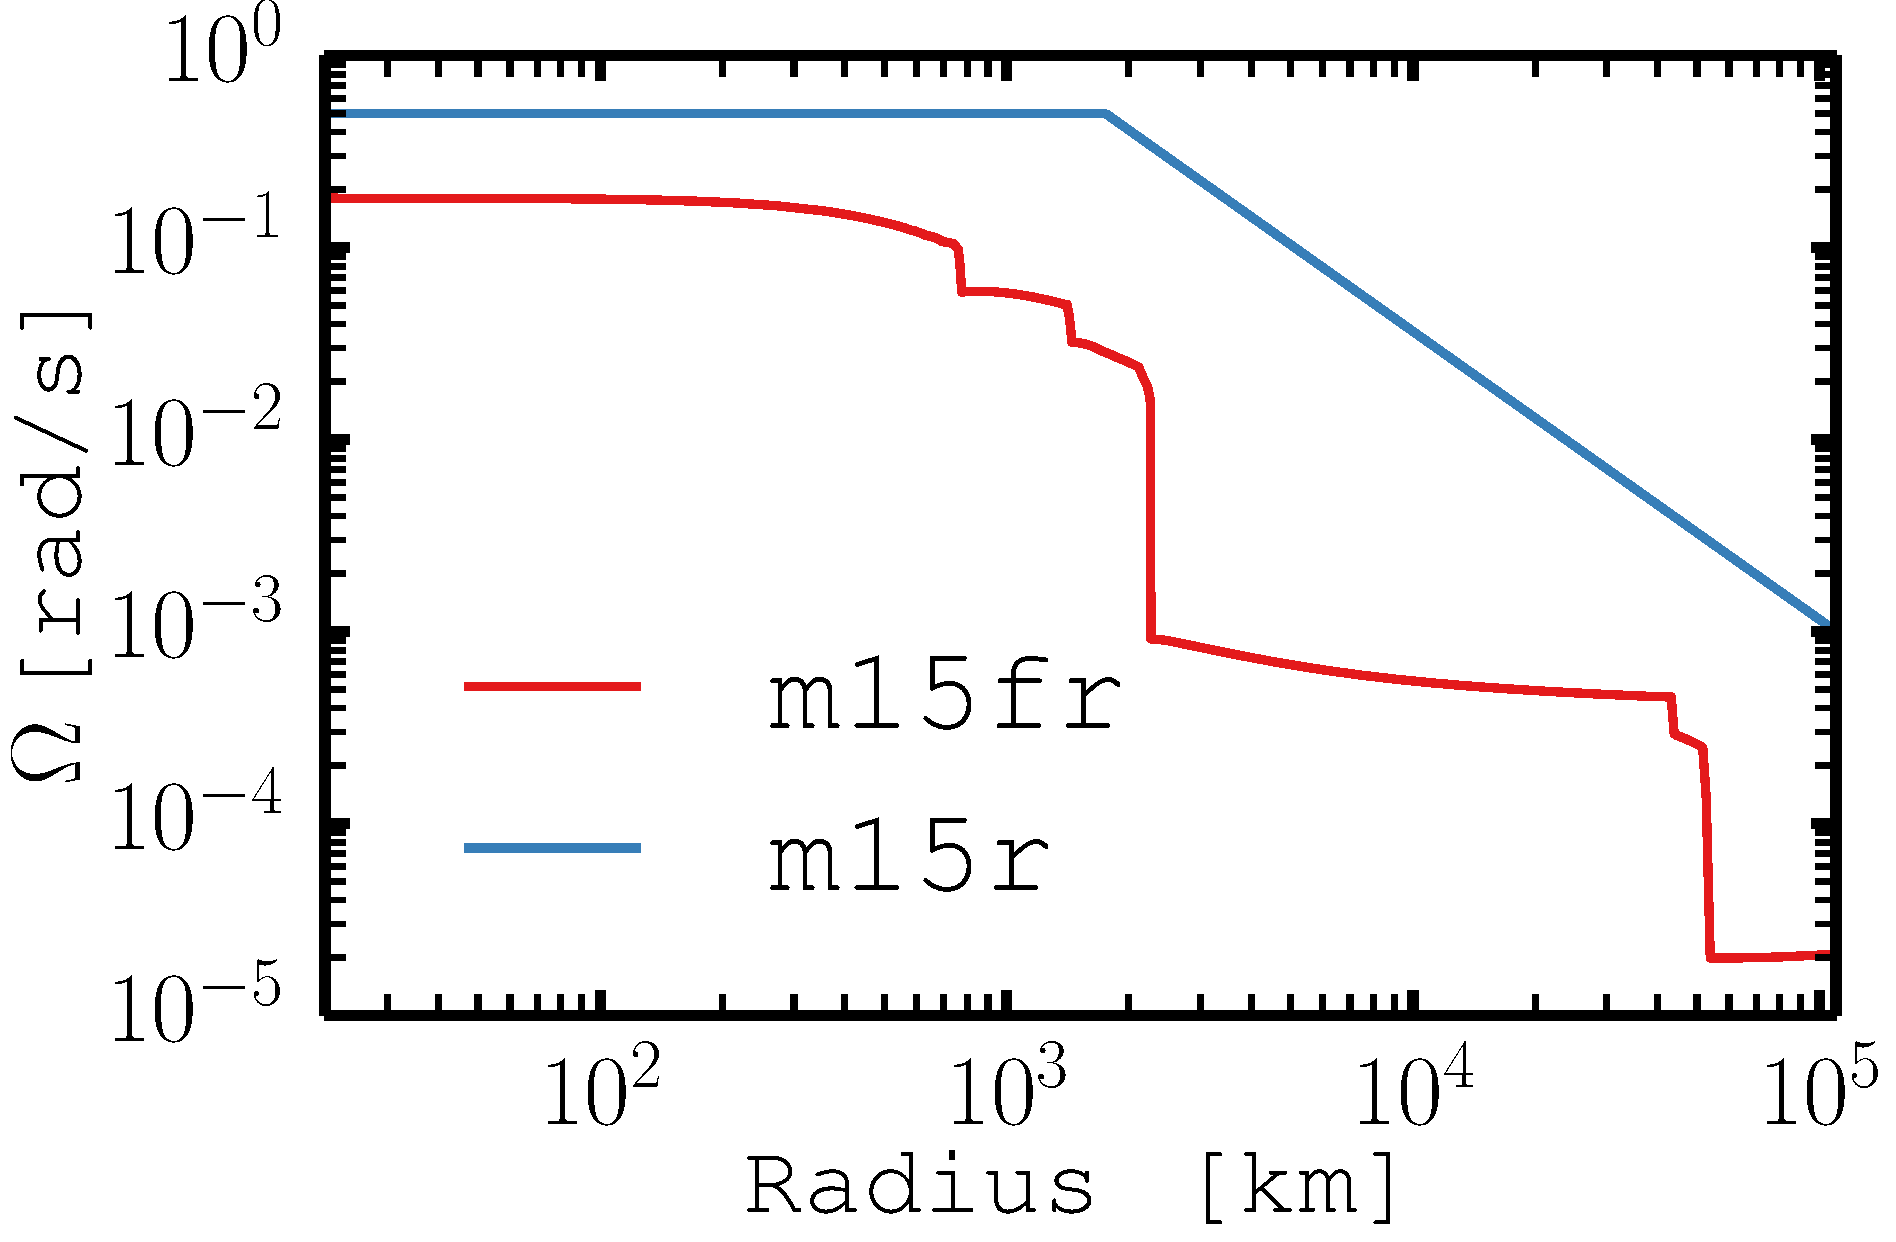
\includegraphics[width=0.99\textwidth]{./images/paper2/rot.pdf}
\caption{The radial rotation profiles for the two rotating models. The blue line represents model 
m15fr and the red line represents m15r. \label{figp2:rot}}
\end{figure}
\begin{figure}[ht]         
\centering                            
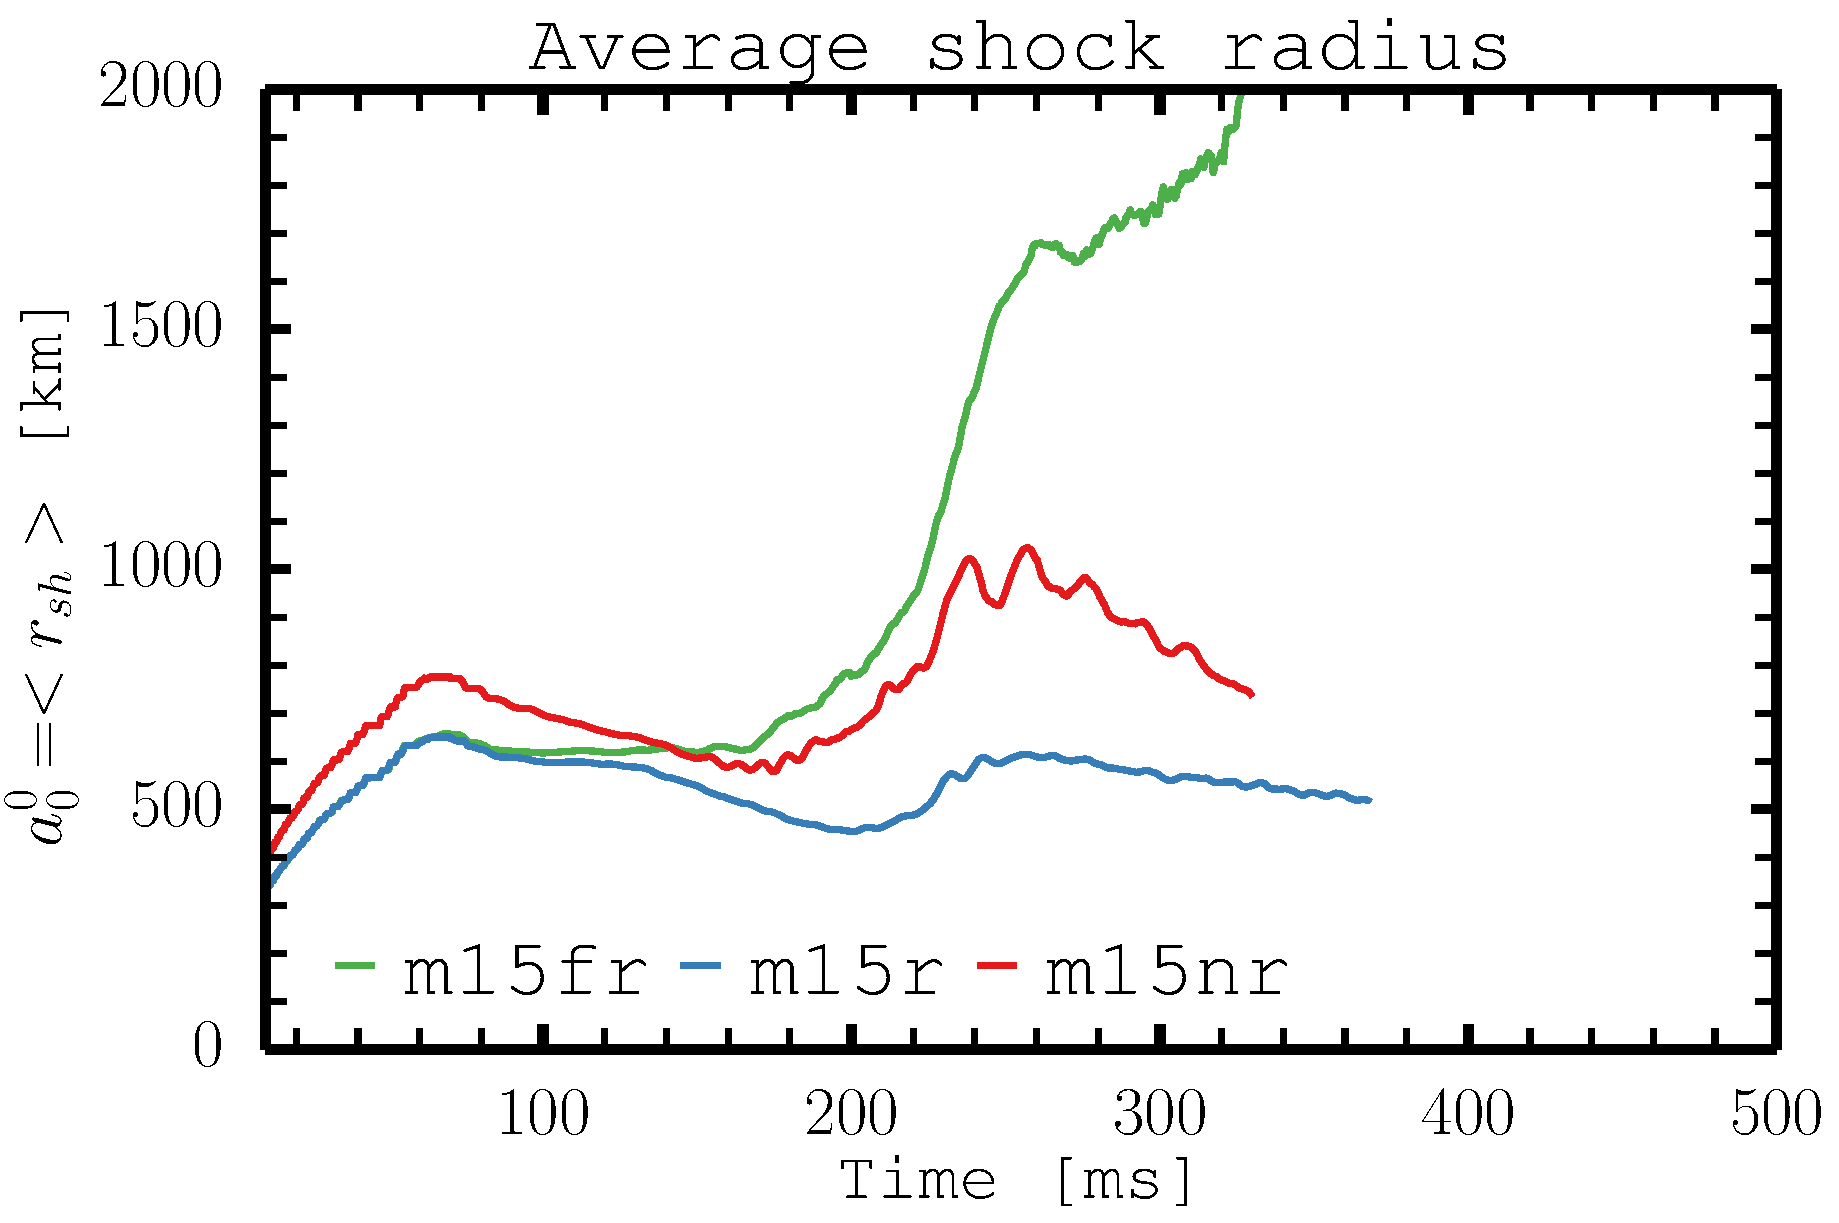
\includegraphics[width=0.99\textwidth]{./images/paper2/rsh.pdf}
\caption{Average shock radius for model m15fr (green), m15r (blue), and m15nr (red) as a function of 
time after core bounce. The average shock radius is defined as the $(l,m) = (0,0)$ expansion coefficient of the shock surface into 
spherical harmonics (\eq{eq:alsph}). \label{figp2:rsh}}
\end{figure}
\begin{figure}[ht]         
\centering                            
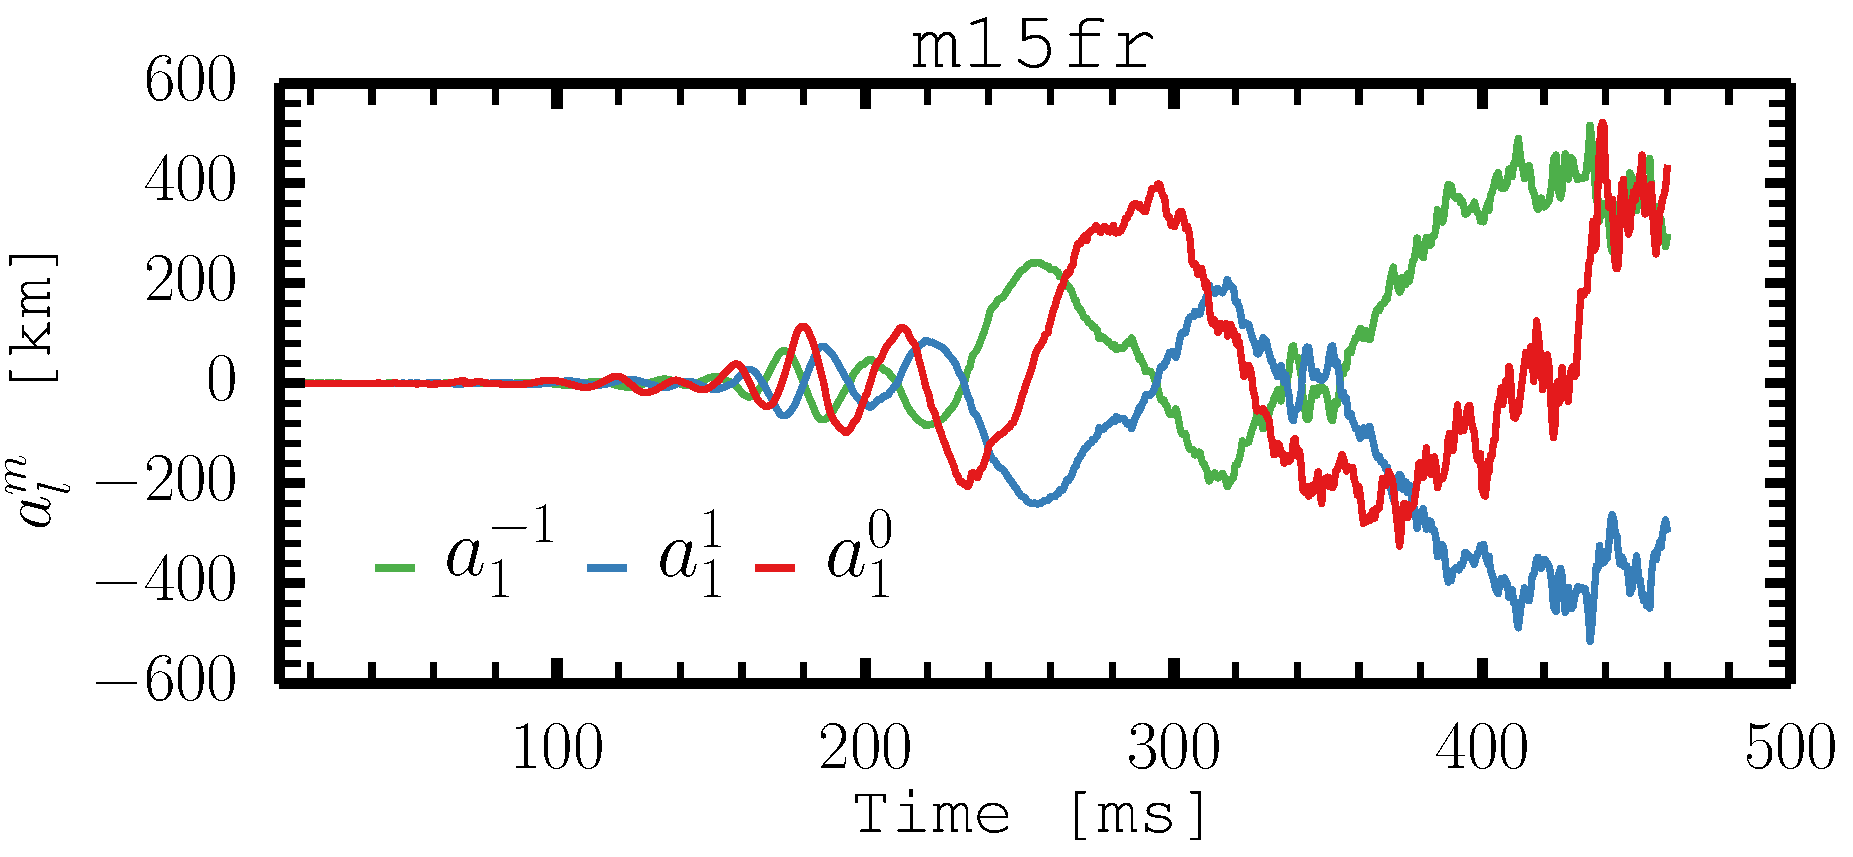
\includegraphics[width=0.9\textwidth]{./images/paper2/sasi_fr.pdf}
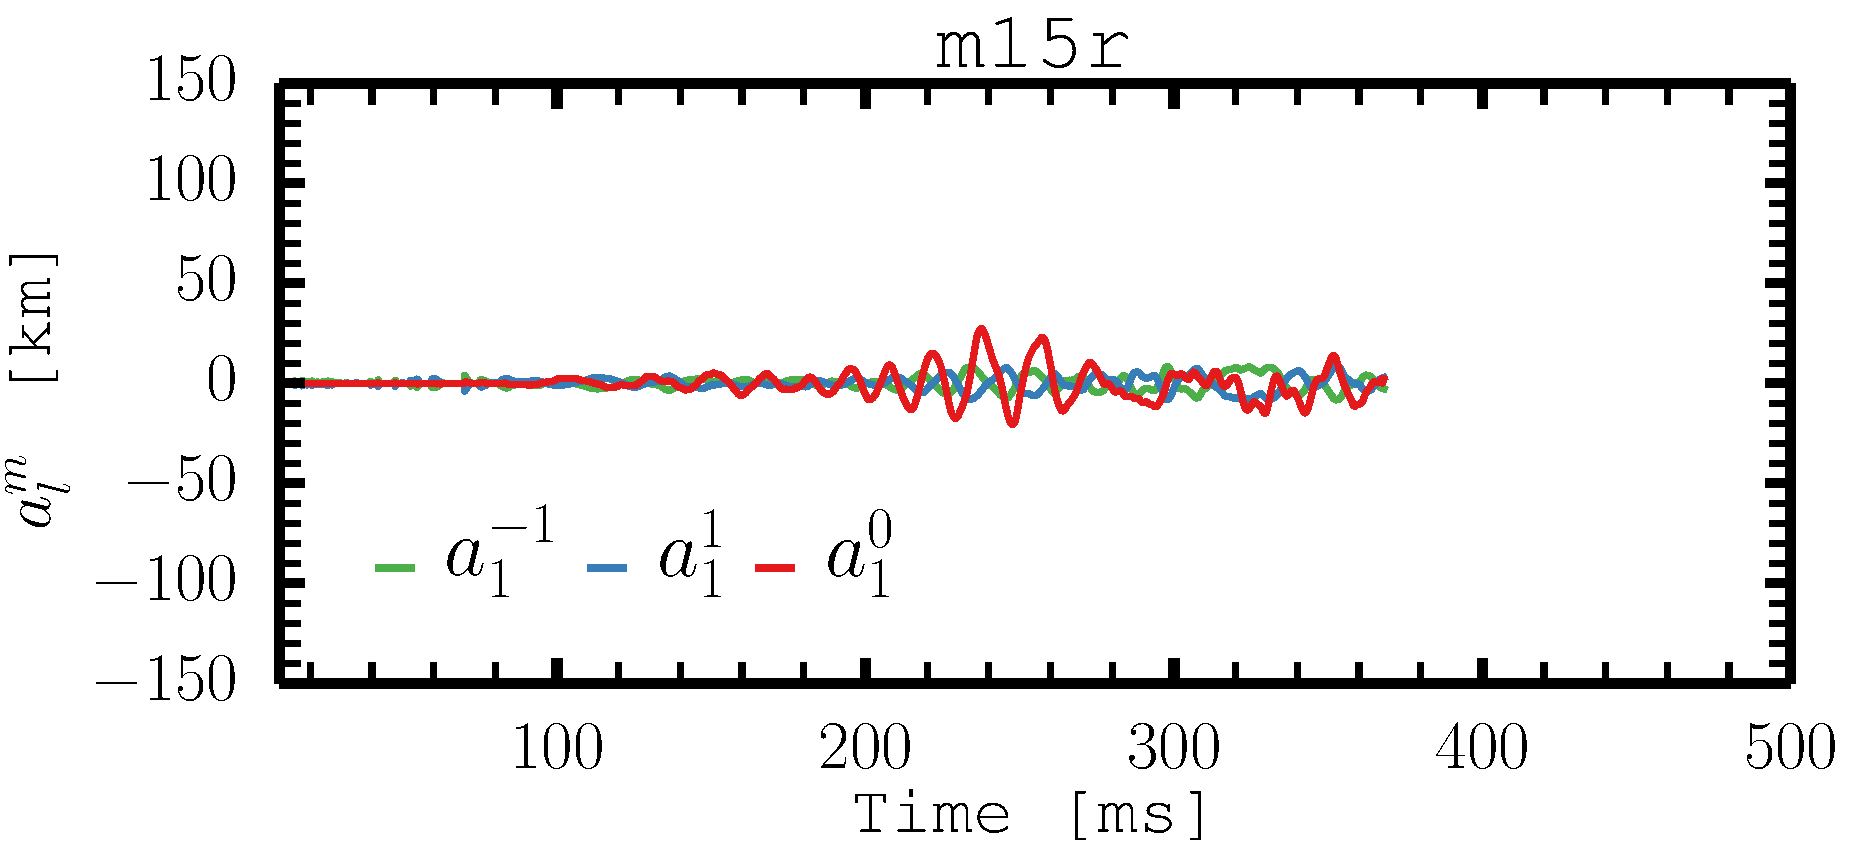
\includegraphics[width=0.9\textwidth]{./images/paper2/sasi_r.pdf}
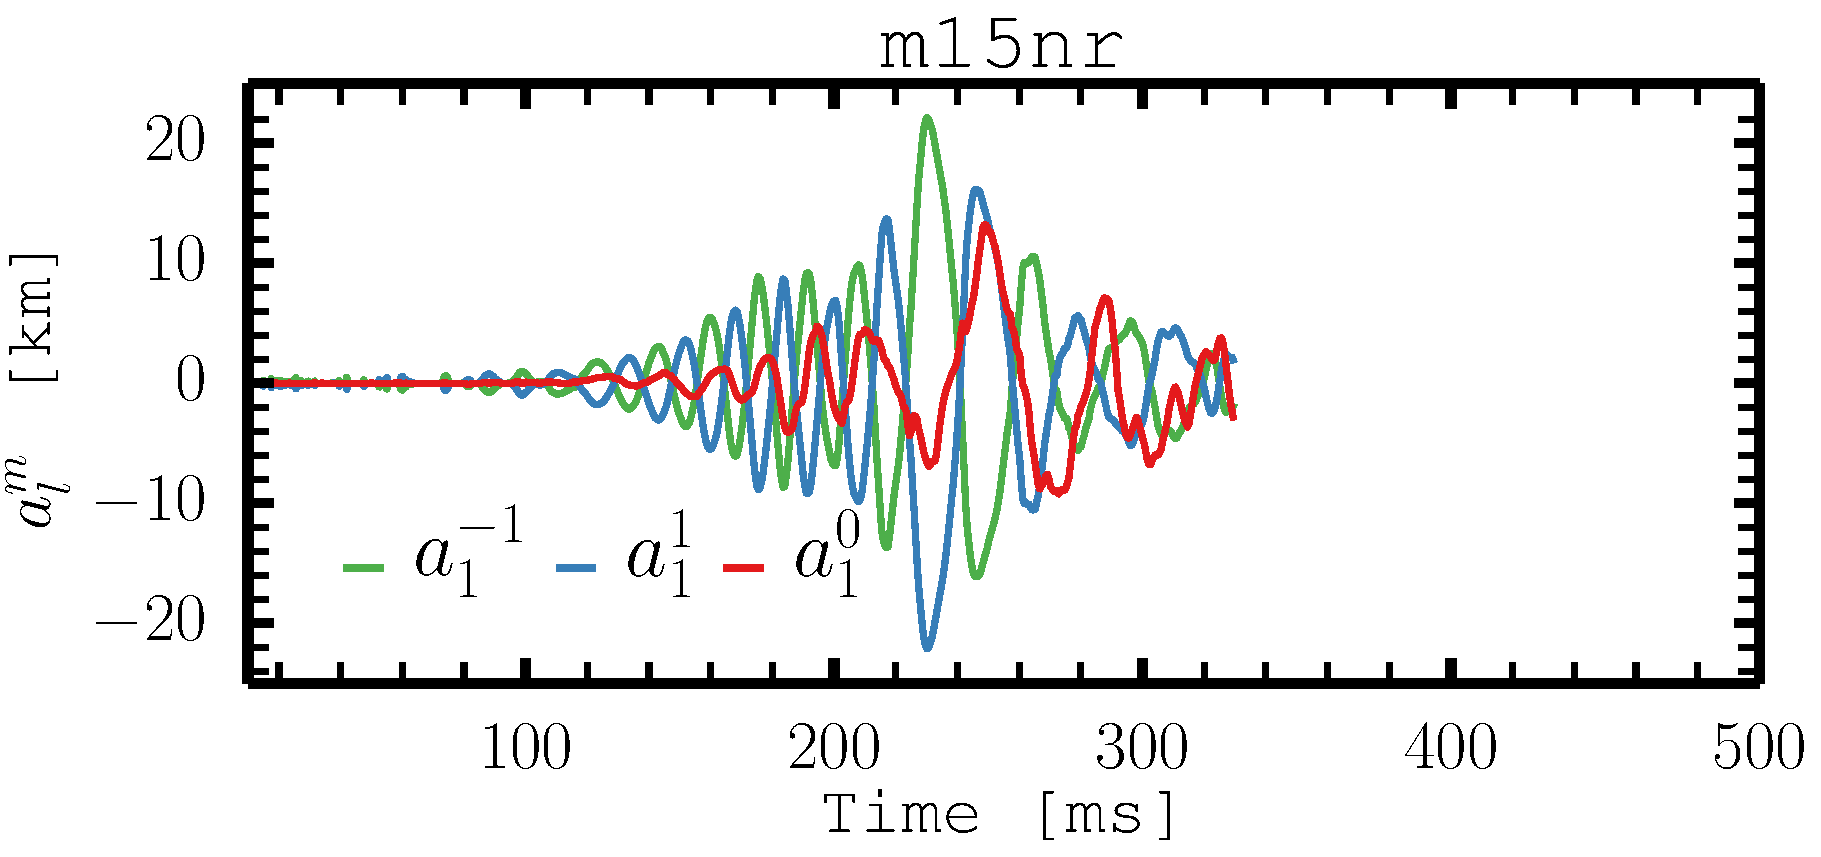
\includegraphics[width=0.9\textwidth]{./images/paper2/sasi_nr.pdf}
\caption{The $(l,m) = (1,0)$, $(1,1)$, and $(1,-1)$ coefficients of the decomposition of the shock surface into spherical harmonics
as a function of time after bounce, see \eq{eq:alsph}. From the top to bottom: Model m15fr, model m15r, and model m15nr. \label{figp2:sasi}}
\end{figure}

\section{Results}
\subsection{Qualitative description of the gravitational wave signals}
The GW signals from the rotating models do not qualitatively differ from
the signals presented in chapter~\ref{ch:firstpaper}. In \fig{figp2:amps} we show the
GW amplitudes generated by asymmetric mass motions for models m15fr, m15r and m15nr.
The two columns show the amplitudes for two different observer orientations,
the right and left column represent observers situated along the x-axis (equator) and z-axis (pole) of the Yin grid-patch,
respectively. The rows are ordered by progenitor, in order of decreasing initial rotation, and from the top
shows m15fr, m1fr, and m15nr. Vertical lines indicate episodes of strong SASI activity.
The corresponding amplitude spectrograms (see \eq{eqSA:STFT}) for a sliding window of $50 \, \mathrm{ms}$ are shown 
in Fig.~\ref{figp2:spec}. The spectrograms show the sum of the squared Fourier
components of the cross and plus polarisation modes,
$\text{STFT}[{A_+}]^2 + \text{STFT}[{A_{\times}}]^2$. Before applying the
DFT we convolve the signal with a Kaiser window with shape parameter $\beta = 2.5$. Frequencies
below $50 \, \mathrm{Hz}$ and above $1100  \, \mathrm{Hz}$ are filtered out of the resulting spectrograms. 

In all three models, an initial phase of quiescence is followed by a phase of stochastic emission, 
during which the typical amplitudes are on the order of a few cm. The fastest rotating model, model m15fr, 
emits the strongest GW signal. 
At the same time the non-rotating model (m15nr) show larger amplitudes than the moderately rotating model (m15r).
There seems to be no clear correlation between the strength initial rotation rate and the strength of the GW emission. 
In the spectrograms (\fig{figp2:spec}) of the three models we see the familiar low-frequency and high-frequency 
components that we saw in the four models presented in chapter~\ref{ch:firstpaper}.

\paragraph{m15fr}
During the SASI phase of m15fr, we see a low-frequency signal 
component in addition to the high-frequency stochastic component. Both strong low-frequency and high-frequency
emission are visible in the upper row of \fig{figp2:spec}. The two signal components
cover a broader frequency range in model m15fr than in the other two models, to the point where the two components almost
overlap. After the shock starts to expand the overall GW amplitudes are strongly reduced, but
both low-frequency and high-frequency emission continues until the end of the simulation.

\paragraph{m15fr}
Of the three models, model m15r produces the weakest GW signal. The GW amplitudes
never exceed $1.5$ cm. Furthermore, the signal is strongly reduced in the
time period between $180$ and $250$ ms post bounce. During this time high-frequency emission
completely subsides and only very weak low-frequency emission is present in the signal.
Around $\sim 250$ ms post bounce high-frequency emission sets in once more, 
at the same time the low-frequency emission ceases. 

\paragraph{m15nr}
The non-rotating model (m15nr) is characterised by a relatively long initial quiescent phase, compared to the two
rotating models. Low amplitude low-frequency GW emission set in around $\sim 125$ ms after bounce. The low-frequency
signal component increases in strength until reaching a maximum around $175$ ms after core bounce.
Approximately $25$ ms after the onset of low-frequency emission, high-frequency emission develops around
$\sim 150$ ms after core bounce. The two signal components remain present in the signal, varying in
strength, until the end of the simulation.

\begin{figure}           
\centering                            
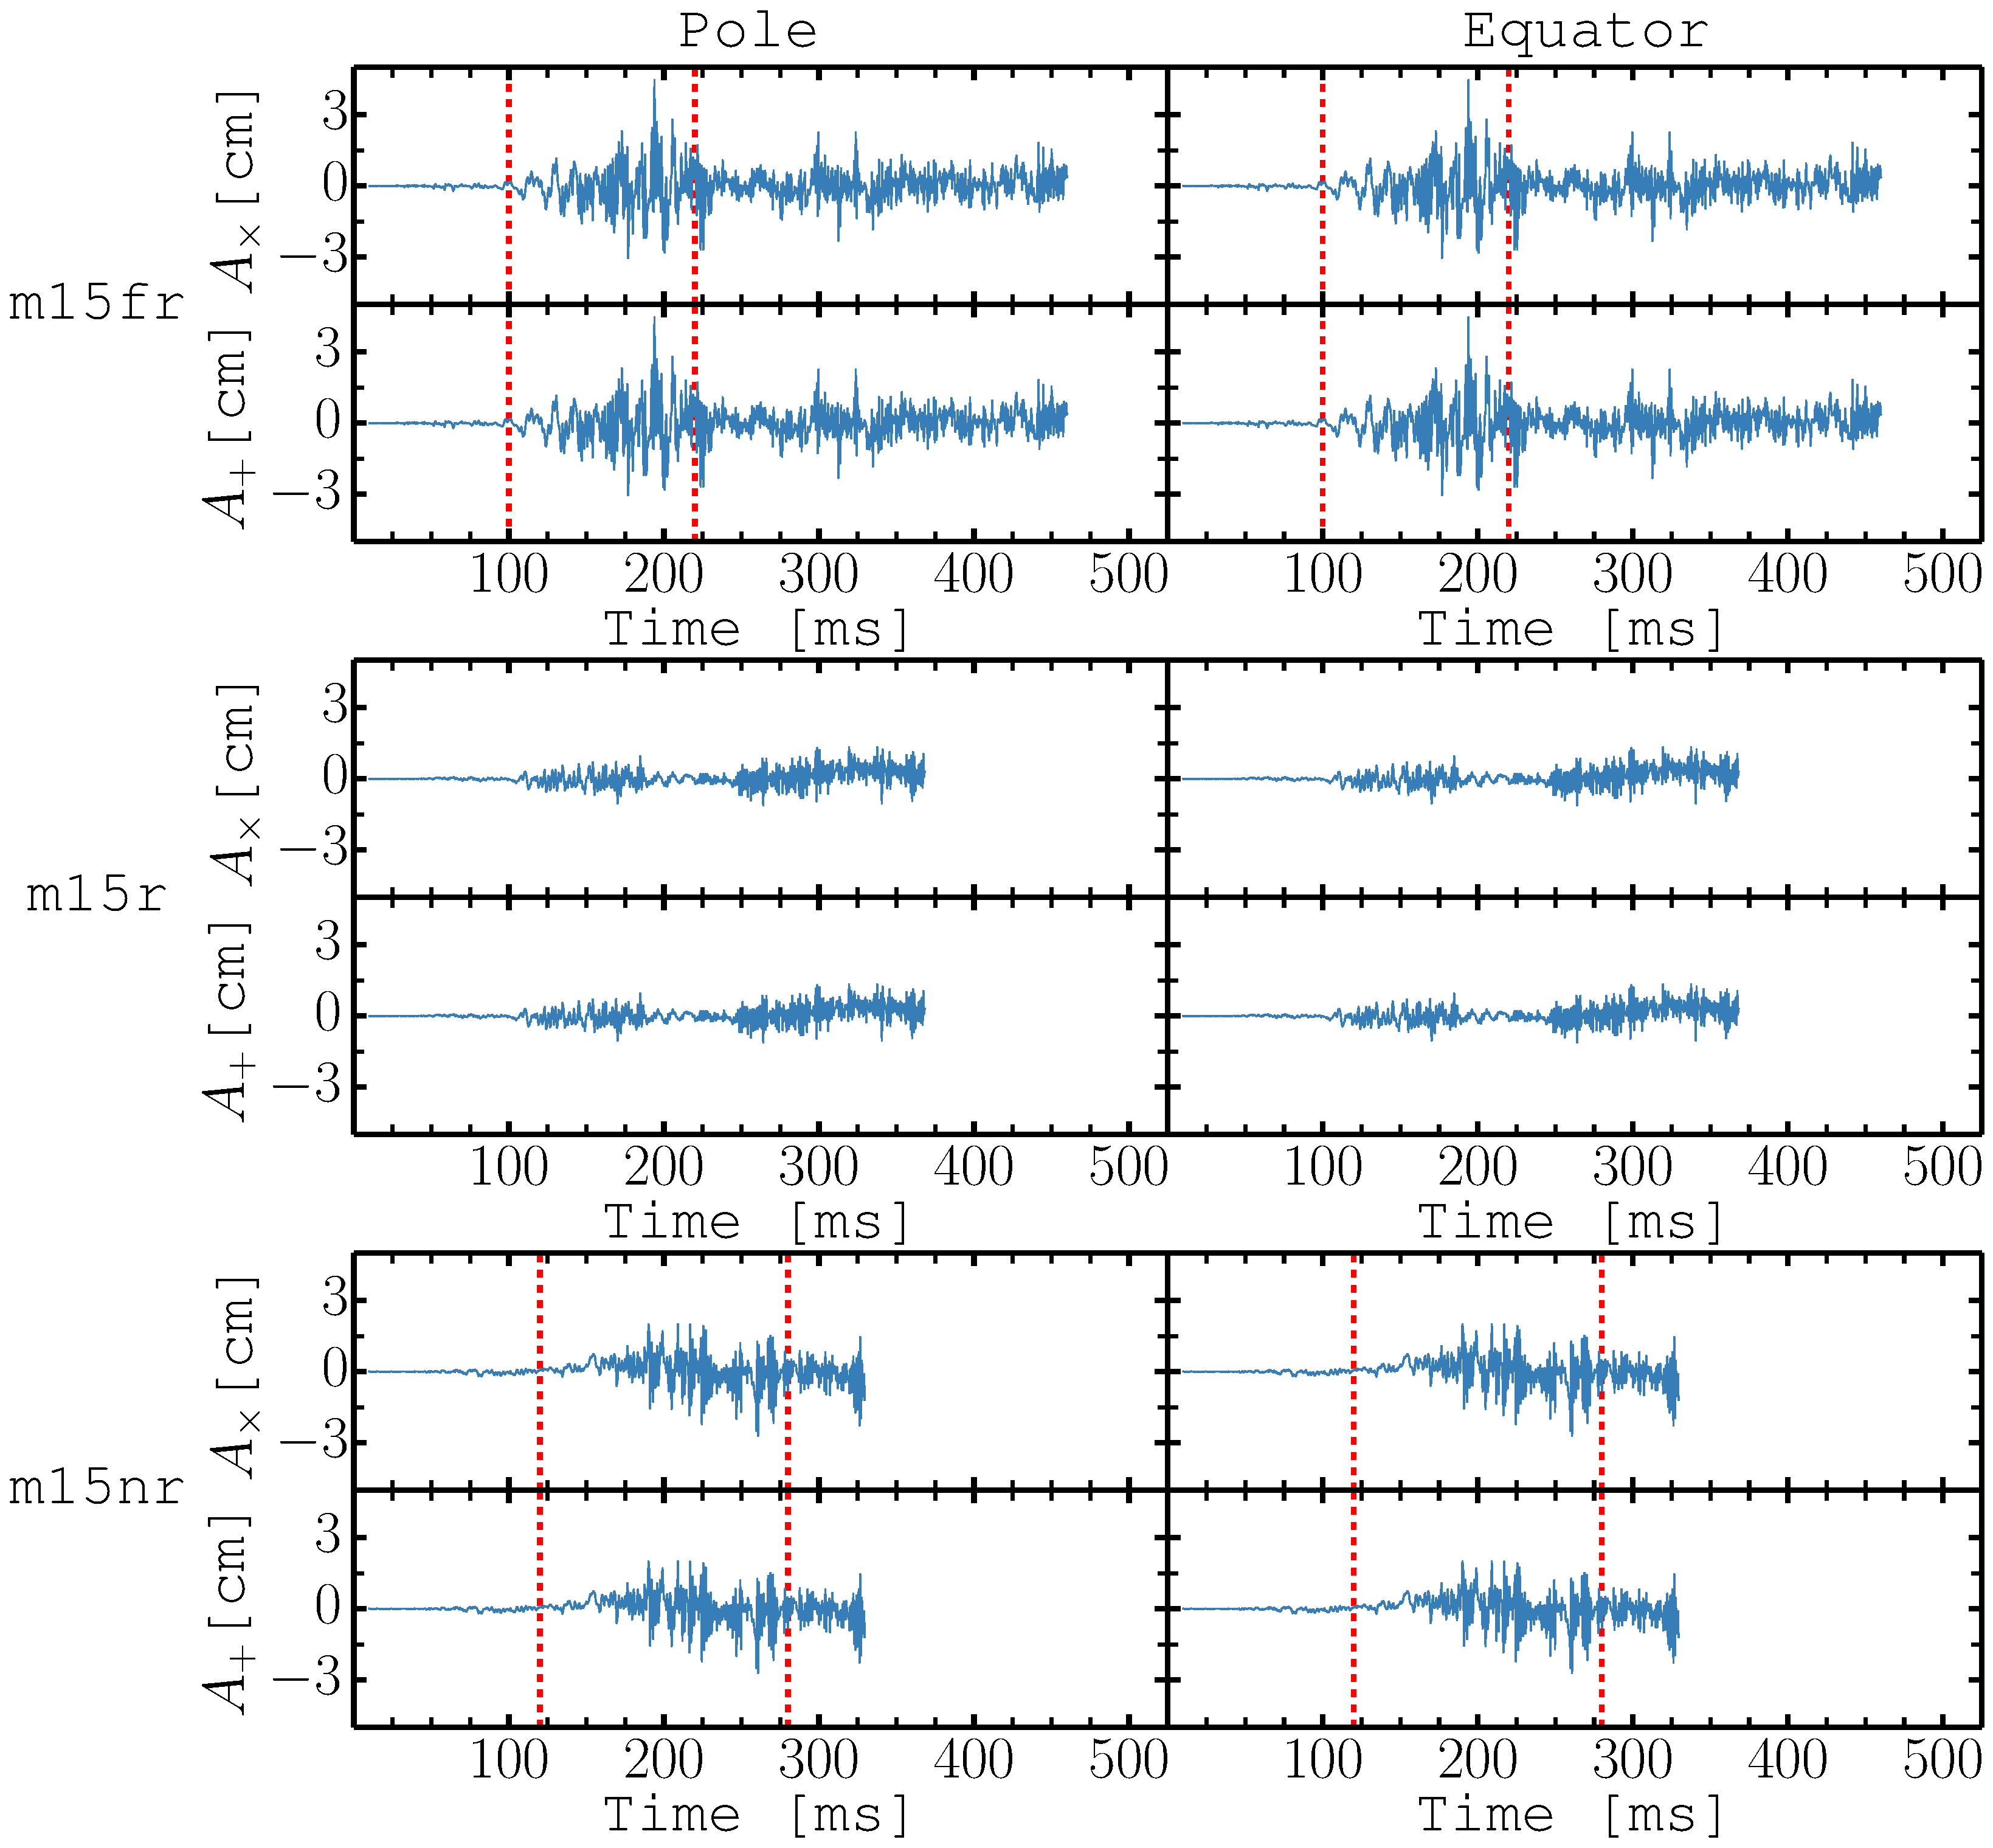
\includegraphics[width=0.99\textwidth]{./images/paper2/amps.pdf}
\caption{GW amplitudes $A_+$ and $A_\times$ as functions of time after core bounce.
  From the top: m15fr, m15r, and m15nr, respectively. 
  The two columns show the amplitudes for two different viewing angles: an observer
  situated along the $z$-axis (pole; left) and an observer situated along the $x$-axis (equator; right) of the Yin grid patch, respectively.
  Episodes of strong SASI activity occur between the vertical red lines.  \label{figp2:amps}}
\end{figure}
\begin{figure}
\centering                            
\includegraphics[width=0.99\textwidth]{./images/paper2/rotspec.pdf}
\caption{Amplitude spectrograms for a sliding window of 50 ms and two different observer
  directions, summed over the two polarisation modes 
  ($|\widetilde{A}_+|^2 + |\widetilde{A}_\times|^2$). The
  different rows show the results for models m15fr, m1fr, and m15nr. (top to bottom).
  The two columns shows the spectrograms for two different viewing angles, the right and left column represent
  observers situated along the z-axis (pole) and x-axis (equator) of the Yin grid, respectively.
  The time is given in ms after core bounce. Vertical lines bracket SASI episodes. All panels have been normalised by the same global factor.
  The colour bar is given in a logarithmic scale. \label{figp2:spec}}
\end{figure}


\subsubsection{Time-integrated energy spectra}
\begin{figure}
\centering                            
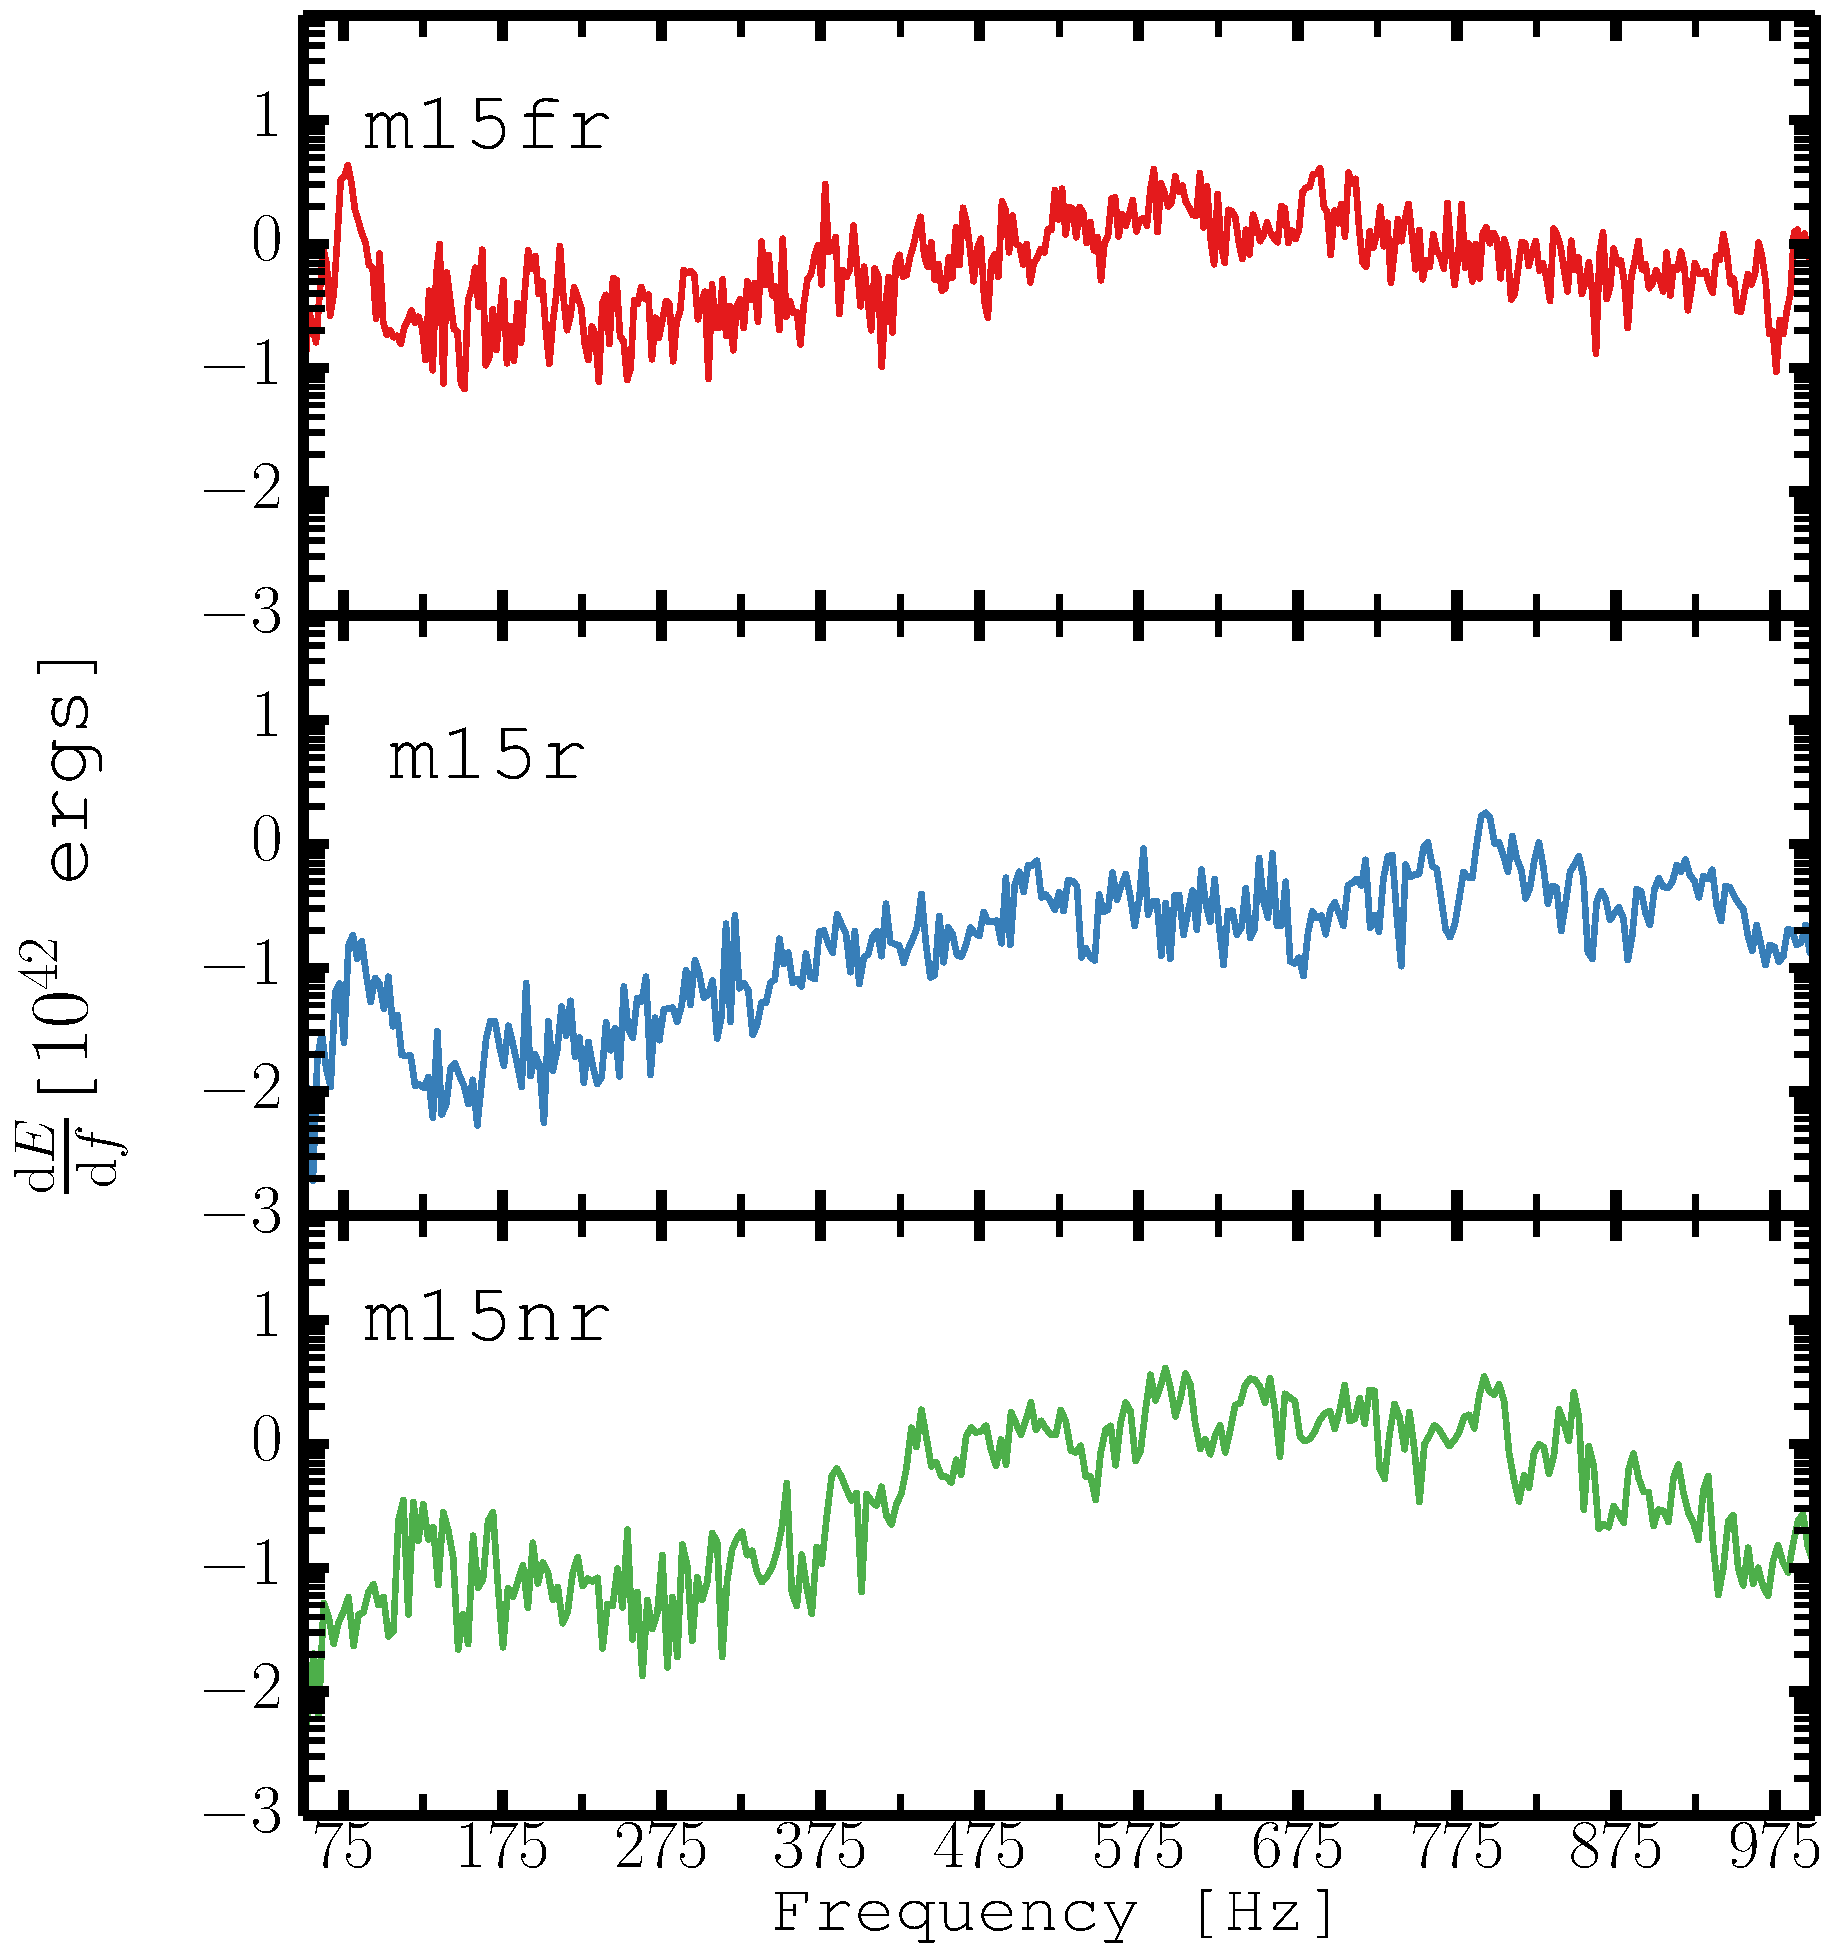
\includegraphics[width=0.79\linewidth]{./images/paper2/dedv_rot.pdf}
\caption{Time-integrated GW energy spectra $\ud E/ \ud f$ for models m15fr,
m15r, and  m15nr (top to bottom). The spectra
are computed from the Fourier transform of the entire waveform
without applying a window function. The y-axis is given in a logarithmic scale.
\label{figp2:energy_spectra}}
\end{figure}
Time-integrated energy spectra for each of the models are shown
in Fig.~\ref{figp2:energy_spectra}. These are computed from
the Cartesian components of the mass quadrupole tensor, according to
\eq{eqT:dedf}.

The time-integrated energy spectrum of model m15fr is rather flat, with strong emission over a wide range of frequencies.
There is a local peak in the spectrum around $\sim 75-100$ Hz. The slower rotating model m15r, which does not
develop strong SASI oscillations, emits much less energy at low frequencies. However, this model also
exhibits a peak in the energy spectrum at frequencies similar to $\sim 75-100$ Hz, but
this peak is much weaker than the one seen in model m15fr.
The energy spectrum of model m15nr is a hybrid between the spectrum of the two previous models. 
As model m15fr, there is a significant amount of energy radiated away by GWs below 300 Hz, but the spectrum is not as flat as the one of model m15fr. 

\section{Excitation of gravitational waves} \label{sec:p2ext}
In chapter~\ref{ch:firstpaper} we studied the hydrodynamic instabilities responsible for GW emission.
We found that GWs are mainly excited in four ways. SASI activity leads to a large-scale asymmetric mass 
distribution in the post-shock layer, that directly leads to strong GW emission. In addition the high-velocity 
violent downflows resulting from SASI activity perturbs the surface PNS surface and excites non-resonant g-modes in the PNS.
Which in turn leads to strong GW emission. The frequency of the forced g-modes 
is set by the typical time scale of the SASI oscillations. High-frequency emission is caused by the propagation of
resonant g-modes outer layers of the PNS. The typical frequency of these oscillations is given by the
Brunt-V\"{a}is\"{a}l\"{a}-frequency in the PNS surface. Resonant g-modes are excited in two ways.
Firstly, by downdrafts from the post-shock layer impinge the PNS surface. Strong downflows can be created by SASI 
activity and overturn of convective plumes. Resonant g-modes are also excited, in the PNS surface layer,
as plumes from the unstable layer beneath overshoot into the surface layer.
For the four models presented in chapter~\ref{ch:firstpaper}, we found that PNS convection was the main driver
of this process, while downflows from the post-shock layer provided a secondary and smaller
contribution (with model dependent variations in the relative importance of the two).

These conclusions hold true for the three models presented in this chapter as well, with one notable
exception. In the two rotating models, model m15fr and model m15r, the GW signal generated by PNS 
convection is significantly reduced. When rotation is added to the simulations a a positive
angular momentum gradient develops in the PNS convection layer, which acts as a stabiliser and weakens PNS
convection \citep{janka_01b}. 
The basic physical picture is that when a buoyant plume propagates outwards its rotation rate
is less than that of the surrounding medium and it experiences a weaker centrifugal force.
The effect of rotation is, therefore, to exact a force acting against the outwards propagation of the plume.
Angular momentum transfer by convection will eventually flatten the rotation profile within the PNS and 
the stabilising effect provided by rotation will gradually decrease with time.

Based solely on the stabilising effects rotation have on PNS convection we would expect an overall 
reduction of high-frequency GW emission in the two rotating models and that the fastest rotating model
emits the weakest high-frequency signal. However, the picture is not
so simple. 
% We have to consider how well the Brunt-V\"{a}is\"{a}l\"{a}-frequency in the PNS surface overlaps with
% the typical SASI and convective time scales. The compactness of the PNS tends to increase with
% progenitor mass, which results in a higher Brunt-V\"{a}is\"{a}l\"{a}-frequency \citep{mueller_13}.
% SASI activity and neutrino-driven convection in the post-shock layer operates at relative long time-scales.
% Consequently, the spectrum of the forcing and the natural g-mode frequency will overlap better
% in model based on a low mass progenitor, with a less compact PNS, than a more massive model. 
% This is in fact reflected in the four models we study in chapter~\ref{ch:firstpaper},
% the contribution to the high-frequency emission by convective plumes striking the PNS from above
% is relative high in model s11.2 (see \fig{fig:cuts}).
We also have to consider the effects of the spiral SASI mode.
The strong influence exerted by the spiral mode on the PNS, through a coherent large-scale
modulation of the accretion flow onto the PNS, not only effectively perturbs the surface, 
but can also reaches into the interior of the PNS and influence the convective layer of the PNS.
A strong spiral SASI mode induces mass motions in the PNS at a set of different frequencies, which is 
reflected in the GW signal as ``broadening'' of both the low-frequency and high-frequency
emission component. This happens because, as mention in the paragraph above, the strong downflows 
created by the SASI does not only excite resonant g-modes, but also forces non-resonant oscillations. 
Model s27, which is dominated by the sloshing mode of the SASI,
has a cleaner emission spectrum than for example the spiral SASI dominated model s20 (see \fig{fig:spectrograms}). Cleaner, in the sense
that the emission is concentrated in narrow bands. The same behavior is seen in model m15fr and
model m15r. A particular strong spiral SASI mode develops in m15fr and this model emit GWs at a
wider range of frequencies than models m15nr, and m15r. 
\begin{figure}[ht]         
\centering                            
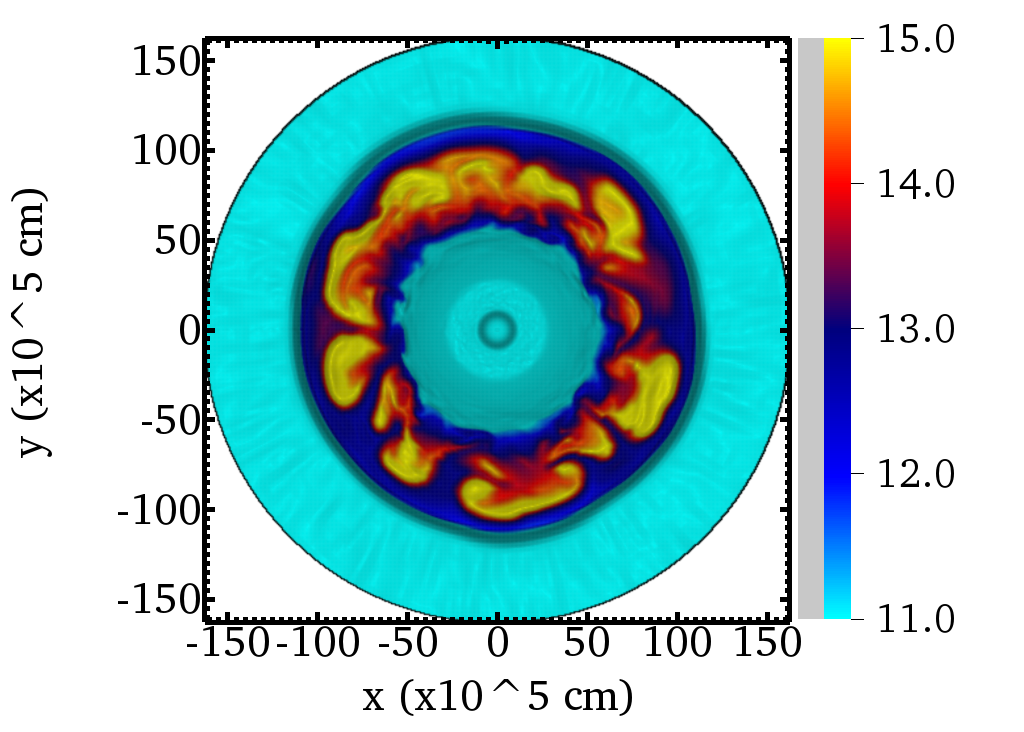
\includegraphics[width=0.49\textwidth]{./images/paper2/1.png}
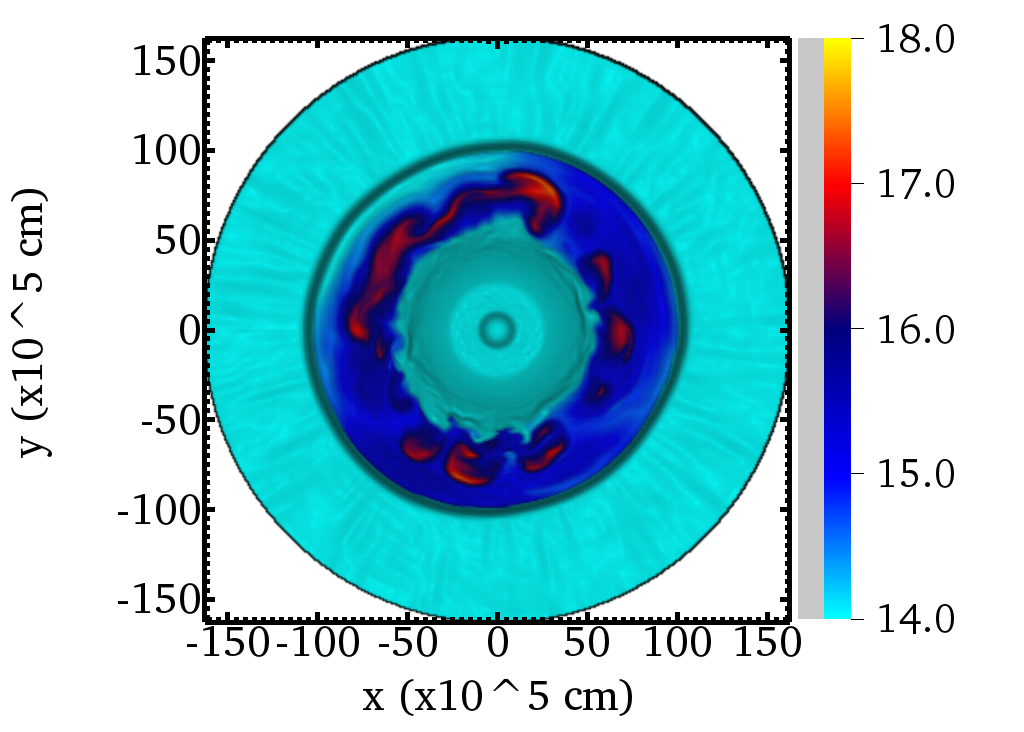
\includegraphics[width=0.49\textwidth]{./images/paper2/2.png} \\
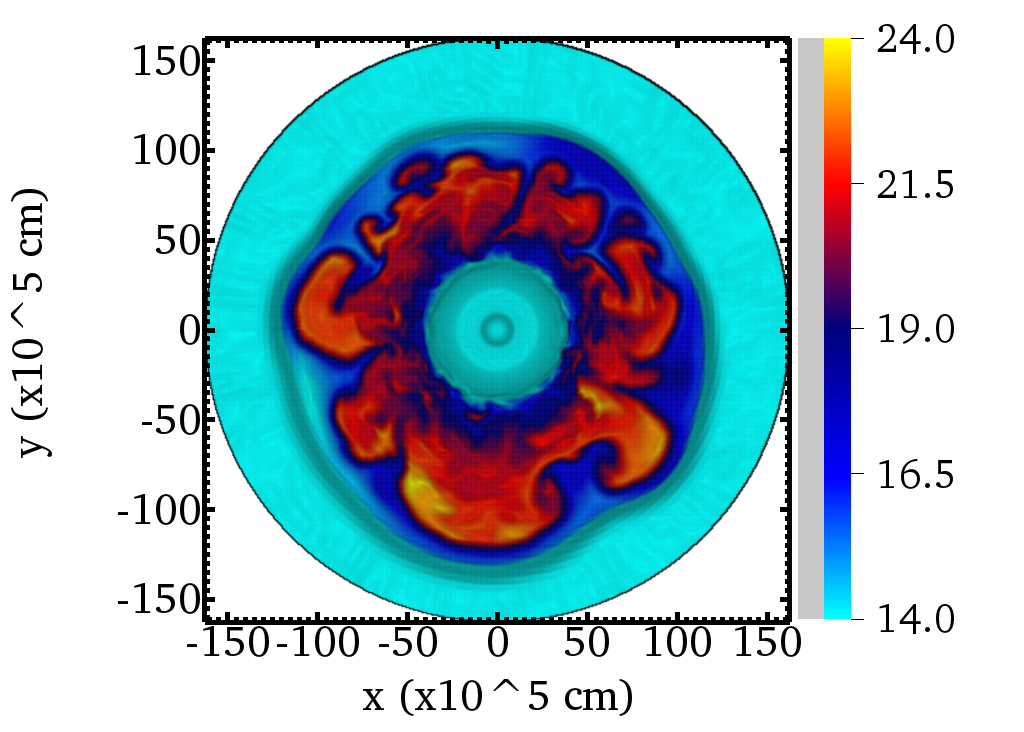
\includegraphics[width=0.49\textwidth]{./images/paper2/3.png}
\caption{The entropy per baryon in the xy-plane of the Yin-grid for model m15r. Shown at
at 167 (top left panel), 210 (top right panel), and 343 (bottom panel) ms post bounce. 
The entropy is given in units of Boltzmann's constant $k_b$. \label{figp2:sto}}
\end{figure}
The reduction of high-frequency GW emission generated by PNS convection can most clearly be seen in model
m15r. Between $180$ and $250$ ms post bounce hot-bubble convection subsidies. During this time
model m15r emits virtually no high-frequency GWs. 
The shock front reaches a minimum around $200$ ms post bounce, after
a $70$ ms long period of recession (\fig{figp2:rsh}). The small average shock radius favours SASI activity over
neutrino-driven convection, and we see the development of low amplitude shock oscillations,
see the middle panel of \fig{figp2:sasi}. Convection, on the other hand, is quenched. 
\fig{figp2:sto} shows the entropy per baryon of model m15r, in the xy-plane of the Yin-grid.
The three panels show snapshots taken 167 (top left panel), 210 (top right panel), and 343 (bottom panel) ms
after core bounce. The top left and the bottom panel show the typical hot bubbles that are characteristic of
neutrino-driven convection, but in the top right panel no such bubbles can be seen. 
The growth of low amplitude SASI activity and the suppression of convection in the post-shock layer is reflected
in the GW signal as weak emission at low frequencies and a complete absence of the high-frequency signal component.
This, naturally, means that high-frequency emission is for the most part caused by convective plumes from
the post-shock layer impinging on the PNS surface.

The reduction of GWs emitted from the PNS can also be seen in model m15fr. After the onset of shock revival
the accretion rate onto the central object decreases and the violent downflows created by strong SASI activity ceases to exist. At the same time there is a strong reduction in the GW signal. This indicates
that excitation of surface g-modes from above is the main source of high-frequency GW emission.
This is in strong contrast to model s20s, where activity within the PNS increased after
the onset of shock revival and consequently led to a strong increase of the GW signal.
This means that the nature of PNS convection is an important factor in determining the 
GW signal from core-collapse supernovae.

\section{The standing accretion shock instability, rotation, and resolution}
In the models we discuss in this chapter, there is no clear connection between the development of SASI activity and the initial rotation rate of
the progenitor. Model m15r, in which the rotation profile is in accord with the stellar
evolution calculations, does not develop strong SASI activity. In both model m15nr and model m15fr, however, a strong spiral SASI mode emerges. 

Exactly how rotation influences the SASI growth rate and saturation does not seem to be a simple function of progenitor rotation rate. Recently \cite{blondin_17} studied the effects of rotation by means of idealised hydrodynamic simulations of a standing accretion shock (in 2D and 3D). 
The results of \cite{blondin_17} are in good agreement with the perturbative study of \cite{yamasaki_08}, 
which found that the linear growth rate 
of non-axisymmetric SASI modes is an increasing function of the progenitor rotation rate.
However, in the non-linear regime \cite{kazeroni_17} does not find a monotonic connection between the
rotation and the saturation amplitude of the SASI. In fact, Fig.3 of \cite{kazeroni_17} indicates that
SASI activity may decrease with increasing rotation rate, at least at low to moderate rotation rates. 

An additional complication comes from the fact that model m15nr was simulated with half the angular resolution of the other two models. The lower resolution has been found
to favour the growth SASI activity, because energy accumulates at larger scales \citep{hanke_12}.
However, \cite{abdikamalov_15} finds the opposite, and conclude that increasing the angular resolution reduces the SASI oscillations. They perform a set of general relativistic 3D hydrodynamic
simulations of a 27 \msun progenitor with a neutrino leakage scheme to study the phase between bounce and
shock revival.

Whether rotation suppresses the growth of SASI activity in model m15r or if SASI activity develops
artificially in model m15nr because of insufficient angular resolution, the absence of strong SASI activity in model
m15r reduces the overall strength of the GW signal. 

\section{Detection prospects}
Following the procedure laid out in section~\ref{sec:obs}, we calculate the possibility of detecting models m15fr, m15r, and m15nr.
In order evaluate the possible of differentiating between models with and without strong SASI activity (strong low-frequency emission)
based on a detection of their GW signals, we compute SNRs in three frequency bands.
The three bands are: the low-frequency band ($f \in [20,250)$, $\delta f= 230$), the
high-frequency band ($f \in [250,1200)$, $\delta f= 950$), and the whole frequency range
($f \in [20,1200)$,  $\delta f= 1180$).
For the three bands we find, by inserting $\delta f$ to \eq{eq:snr_band2} and assuming that the
signal length $\Delta t \sim 0.5$, detection thresholds of $\mathrm{SNR}_\mathrm{low} \gtrsim 11$, 
$\mathrm{SNR}_\mathrm{high} \gtrsim 15$, $\mathrm{SNR}_\mathrm{whole} \gtrsim 20$ for the
low-frequency band, the high-frequency band, and ``whole-frequency'' band, respectively.
As in chapter~\ref{ch:firstpaper}, we calculate the SNR from Eq.~(\ref{eq:snr}) for the zero-detuning-high power configuration
of Advanced LIGO \citep{adv_sens} and the B \citep{et_b} and C \citep{et_c} configurations for the Einstein
telescope. These configurations are referred to as as AdvLIGO, ET-B and ET-C.
\begin{table}[]
\caption{Signal-to-noise ratio for models m15fr, m15r, and m15nr. Values
are given for two different frequency domains, $20\ldots 250 \, \mathrm{Hz}$
(low-frequency), $250\ldots 1200 \, \mathrm{Hz}$ (high-frequency), and
for the whole frequency domain, $20 \ldots 1200$. 
The table shows values for two different
detectors, AdvLIGO and the Einstein Telescope. 
For the latter, we calculate the SNR for two
different modes of operation (ET-B and ET-C). The table shows SNRs for a source at a distance of $10 \, \mathrm{kpc}$. 
The three tables show SNRs for model m15fr, model m15r, and model m15nr (from top to bottom). 
\label{tablep2:SNR}}
\begin{subtable}{.95\linewidth}
\centering
\vspace{.5 cm}
\begin{tabular}{>{\centering}m{5cm}|>{\centering}m{1.5cm}|>{\centering}m{1.5cm}|>{\centering}m{1.5cm}|l}
\multicolumn{1}{l|}{m15fr}   & Low   & High & Total & Low/High \\ \hline
\multicolumn{1}{l|}{AdVLIGO} & 10.8  & 4.9  & 11.9  & 2.20          \\ \hline
\multicolumn{1}{l|}{ET-C}    & 133.2 & 67.6 & 149.4 & 1.97          \\ \hline
\multicolumn{1}{l|}{ET-B}    & 224.6 & 83.5 & 239.6 & 2.69          \\ 
\end{tabular}
\end{subtable}
\newline
\vspace{.5 cm}
\newline
\begin{subtable}{.95\linewidth}
\centering
\begin{tabular}{>{\centering}m{5cm}|>{\centering}m{1.5cm}|>{\centering}m{1.5cm}|>{\centering}m{1.5cm}|l}
\multicolumn{1}{l|}{m15r}     & Low  & High & Total & Low/High \\ \hline
\multicolumn{1}{l|}{AdVLIGO}  & 2.6  & 2.4  & 3.5   & 1.08          \\ \hline
\multicolumn{1}{l|}{ET-C}     & 32.2 & 34.4 & 47.1  & 0.93          \\ \hline
\multicolumn{1}{l|}{ET-B}     & 53.7 & 41.1 & 67.7  & 1.30          \\ 
\end{tabular}
\end{subtable}
\newline
\vspace{.5 cm}
\newline
\begin{subtable}{.95\linewidth}
\centering
\begin{tabular}{>{\centering}m{5cm}|>{\centering}m{1.5cm}|>{\centering}m{1.5cm}|>{\centering}m{1.5cm}|l}
\multicolumn{1}{l|}{m15nr}   & Low  & High & Total & Low/High \\ \hline 
\multicolumn{1}{l|}{AdVLIGO} & 3.5  & 4.3  & 5.5   & 0.81     \\ \hline
\multicolumn{1}{l|}{ET-C}    & 46.5 & 59.3 & 75.2  & 0.78     \\ \hline
\multicolumn{1}{l|}{ET-B}    & 74.0 & 72.0 & 103.2 & 1.02     \\ 
\end{tabular}
\end{subtable}
\end{table}

In the low-frequency band the SNR of model m15fr is roughly equal to that of model s20s in the low-frequency band, for
all the three detector configurations. The strong spiral SASI activity and the reduced high-frequency emission,
due to dampening of PNS convection by rotation, leads to a high ratio between the $\mathrm{SNR}_\mathrm{low}$
and $\mathrm{SNR}_\mathrm{high}$. Model m15r shows that one has to be careful when interpreting the ratio $\mathrm{SNR}_\mathrm{low}/\mathrm{SNR}_\mathrm{high}$. The reduction of the high-frequency emission and
the presence of, due to intermediate and weak SASI activity, leads to ratios of $\mathrm{SNR}_\mathrm{low}/\mathrm{SNR}_\mathrm{high}$
which are $\sim 15-25$ higher than those of model m15nr, for all three detector configurations. However, model m15nr clearly develops much stronger SASI activity than model m15r. This means that an excess of power in the low-frequency band might not be a
clear indicator of strong SASI activity.

At a distance of 10 kpc, none of our models would be detectable with AdVLIGO. For the Einstein telescope the situation is
significantly better. We estimate that model m15fr should be debatable out to distances of 75 kpc, while model m15nr
and model m15r could be detected at $\sim 20$ kpc and $\sim 30$ kpc, respectively. The B configuration of the detector shows the most
promise and can effectively increase those numbers by $\sim 35-60\%$. 

\section{Conclusion and discussion}
In this chapter, we studied progenitor rotation affects the GW signal of core collapse supernovae.
We have not studied rapidly rotating models, but we have rather focus the regime of moderate progenitor rotation.
Our main findings are:
\begin{enumerate}
\item Moderate rotation does not change the frequency structure of the GW signal, compared to the signal from non-rotating models.
We see the familiar two-component structure with a high-frequency and a low-frequency signal component.
\item We find that the high-frequency emission instigates by PNS convection in weaker in the rotating models. This is because rotation has a stabilising effect on PNS convection and decreases the amount of energy dissipated in the overshooting region PNS.
This becomes particularly apparent in model m15r, in this model we find a strong reduction of the GW amplitudes during a 
period of time when post-shock convection is weak. The generally weak amplitudes in this model reaffirm the fact that post-shock convection is a weak source of GW excitation, compared to PNS convection and SASI activity.
\item Of the three models presented in this chapter the fastest rotating model emits the strongest GW signal, this is
because this model develops the strongest spiral SASI mode. Based on the models presented here one should not conclude
that the strength of the signal will increase with increasing progenitor rotation rate. The conclusion should instead be
that the stronger the spiral mode of the SASI is the larger the amplitudes of the GW signal are. However, it is not clear
that stronger rotation leads to stronger SASI activity.
\item It should be emphasised that model m15r, where the rotation rate is exactly in accordance with the stellar evolution
calculations of the 15 \msun progenitor these three models are based on, shows the weakest GW signal.  
\item Unlike model s20s, the GW signal of model m15fr decreases after the onset of shock revival. This reduction is due to
the small contribution to the total signal from mass motions instigated by PNS convection.
\end{enumerate}

The GW signal from rapidly rotating models have been studied 
by several authors \citep{mueller_82,rampp_98,shibata_05,ott_05,scheidegger_10,kuroda_14,takiwaki_16}. 
A common feature of these studies is that they tend to predict rather strong emission of gravitational radiation. During the post-bounce phase rapid rotation can lead to the
development of novel flow patterns that are not observed in slow/non-rotating models.
\cite{rampp_98} and \cite{shibata_05} found that very rapid rotation can
lead to a bar-like deformation of the central core. In the somewhat slower 
rotating models of \cite{ott_05}, \cite{kuroda_14}, and \cite{takiwaki_16} the development of
a low-mode spiral instability was found. These asymmetric and rapidly rotating structures
lead to strong GW emission. 

Because of the strong and fairly monochromatic GW emission predicted by these models,
it is predicted that such events should be detectable even at large distance. \citep{gossan_15} found that the
most extreme case would be detectable with Advance-LIGO at a distance of over 3 Mpc. On the other, hand
the models presented in this thesis would be with Advance-LIGO at distances of a few kpc. 
It is, however, not likely that a large part of the core collapse supernovae progenitors
have rapidly rotating, or even moderately rotating, cores. Observations of pulsars put
strong constraints on the rotation rate of core-collapse progenitors. It has been estimated that
most pulsars are formed with rotation periods of a few tens to hundreds of milliseconds \citep{vranesevic_04,popov_12,noutsos_13}.
The recent study of \cite{kazeroni_17} concludes that
the one armed-spiral instability \citep{ott_05,kuroda_14,takiwaki_16} is not able to spin down the PNS enough to make rapidly rotating progenitors compatible with the spin rate of young
pulsars. Additionally, stellar evolution models which include the effects of magnetic files predicts
slowly rotating stellar cores \citep{heger_05}. Results from asteroseismology \cite{beck_12,mosser_12} indicates
that the cores low-mass red giants rotate slower than what was expected from stellar evolution \citep{cantiello_14,deheuvels_14}.
According to results from asteroseismology, angular momentum loss due to stellar winds seems to play a bigger role than currently predicted by stellar evolution calculations \citep{cantiello_14}. 

The rotation rates of the two rotating models studied here is more along the lines of what 
is expected from sate of the art stellar evolution calculations \citep{heger_05} and observations 
\citep{beck_12,mosser_12,popov_12,noutsos_13,cantiello_14,deheuvels_14}. 
We find no quantitive difference between the GW signals from rotating models and we must conclude that
a stochastic signal with amplitudes of few cm seems to be the generic core-collapse GW signal.
Which leads to the conclusion that moderate to low progenitor rotation will not significantly increase the detectability of 
GWs from core-collapse supernovae. In fact, it might be that rotation decreases the signal strength and consequently make them harder to detect. 

The fact model m15nr, the non-rotating model, has an angular resolution that is two times lower
(four versus two degrees) than the two other models makes it difficult to draw strong conclusions about how low-frequency signal changes with increasing rotation. It might be that model m15nr
develops an artificially strong spiral SASI mode due to the lower resolution, but it is also possible that rotation quenches the spiral mode in model m15r. Another weakness of our study is that the three
models are all start from a from spherically symmetric progenitor models. 
It is not realistic to expect starts to be perfectly spherical symmetric objects.
It has, in fact, been found that asymmetries in the burning shells of the progenitor can influence the shock dynamics and even help to ensure a
successful explosion \citep{burrows_96,fryer_04,arnett_11,couch_13,mueller_15a}. In a rotating progenitor, such inhomogeneities could lead to a sizable emission of GWs
during the collapse and right after core bounce. The long period of quiescence after bounce could be an artifact of the spherical symmetric progenitors.



% Whether a significant proportion of supernova progenitors have moderately rotating (let alone rapidly rotating) cores is unclear. 
% Predictions of the initial rotation rate of pulsars, based on their current
% spin-down rate and age, suggest that a large fraction of the pulsar population is born 
% with rotation periods of the order of tens to hundreds of milliseconds \citep{popov_12,noutsos_13}. 


% Stellar evolution models that include the effects of magnetic fields predict rather slowly rotating
% pre-collapse cores \citep{heger_05}. Furthermore, the angular momentum loss due to stellar winds 
% seems to be underestimated by stellar evolution models, compared to results from asteroseismology \citep{cantiello_14}.
% Predictions of the initial rotation rate of pulsars, based on their current
% spin-down rate and age, suggest that a large fraction of the pulsar population is born 
% with rotation periods of the order of tens to hundreds of milliseconds \citep{popov_12,noutsos_13}. 
